%!TEX root = volumeFinal.tex 
\chapter{\label{chap:ativ}Jogos}

Jogos eletrônicos são muito populares, principalmente pela grande quantidade de gêneros, existem jogos de ação, aventura, esportes, estratégia, entre outros. Hoje em dia, os jogos buscam que quem jogue consiga ficar imerso no dentro do jogo, sem conseguir identificar um padrão nos jogadores fictícios, pois se não o jogo deixa de ser tão interessante. Para que isso aconteça, a IA é associada a diversos jogos, e é comum pensar que quanto mais complexa a IA aplicada dentro do jogo mais difícil jogo irá ficar, mas isso nem sempre é verdade. Não é sempre que uma IA complicada terá melhor desempenho do que uma mais simples. Uma boa IA, para jogos, é feita a partir do comportamento desejado para o jogo com os algoritmo certos~\cite{millington2009artificial}.

\section{Jogos de estratégia em tempo real}

Jogos de estratégia em tempo real, também conhecido por \textit{real-time strategy games} (RTS), é um subgênero de jogos de estratégia. Nesse gênero de jogo os jogadores precisam ter uma economia dentro do jogo, e com isso devem construir uma base, buscar recursos, construir edificações, treinar unidades de ataques e aprimorar suas tecnologias. Mas no final, o objetivo do jogo é destruir uma ou mais bases inimigas~\cite{ontanon2013survey, buro2012real}. 

Existem algumas diferenças entre jogos RTS e jogos de tabuleiro, como xadrez. Estas diferenças são~\cite{ontanon2013survey}:

\begin{itemize}
	\item movimentos simultâneos, jogadores realizam jogadas ao mesmo tempo;
	\item tempo real, cada jogador deve realizar suas ações em um curto espaço de tempo;
	\item parcialmente observável, na maioria dos jogos RTS, o jogador só consegue enxergar parte do ambiente;
	\item não-determinístico, nem sempre uma ação realizada resulta na saída esperada; e
	\item complexidade, o espaço de estados e o número de ações possíveis é muito grande.
\end{itemize} 

Pelo fato de existirem essas diferenças, não é possível traduzir automaticamente as técnicas padrões dos jogos de tabuleiro para jogos RTS sem algum tipo de abstração ou simplificação~\cite{ontanon2013survey}.

\section{MicroRTS}  

Um exemplo deste gênero é o MicroRTS\footnote{https://github.com/santiontanon/microrts}, uma simplificação de jogos como Starcraft\footnote{http://us.battle.net/sc2/pt/}. O MicroRTS foi feito por Santiago Ontañón~\cite{ontanon2013combinatorial} em Java. O MicroRTS foi desenvolvido para fins acadêmicos, com o intuito de aplicar e desenvolver técnicas de IA e para servir como prova de conceito para as técnicas criadas.

\begin{figure}[ht]
	\centering
	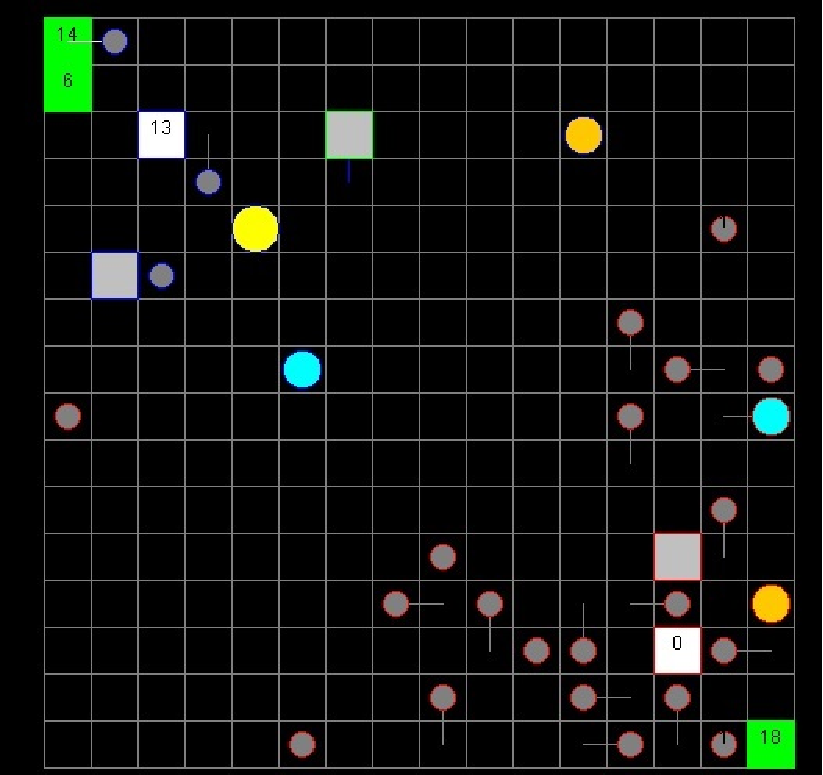
\includegraphics[width=0.5\textwidth]{fig/microrts.pdf}
	\caption{Um exemplo de tela do MicroRTS}
	\label{fig:microrts}
\end{figure} 

O MicroRTS consiste em dois jogadores tentando destruir a base adversaria. Para destruir com o inimigo é preciso eliminar cada unidade e edificações adversarias. A Figura~\ref{fig:microrts} mostra um exemplo de tela do jogo.
No MicroRTS existem quatro tipos de unidades no jogo, e cada uma foi descrita a seguir:

\begin{itemize}
	\item \textit{worker}, é responsável por coletar recursos e construir as edificações. Esta unidade também consegue lutar, mas possui um dano muito baixo;
	\item \textit{heavy}, unidade que pode apenas atacar. Ela possui um alto poder de ataque, mas sua velocidade é lenta;
	\item \textit{light}, unidade que pode apenas atacar. Ela possui um baixo poder de ataque, mas sua velocidade é rápida; e
	\item \textit{ranged}, unidade que pode apenas atacar. Ela possui um ataque de longa distância. 
\end{itemize} 

Para treinar as unidades é preciso ter recursos e edificações. No MicroRTS é preciso ter uma base que é a edificação principal. Ela é responsável pela criação dos \textit{workers}, e nela também é guardado os recursos coletados pelos \textit{workers}. Ela é de grande importância, pois é apenas nela que é possível armazenar os recursos, que são necessários para treinar e construir tudo dentro do jogo. O quartel é responsável pela criação das unidades de ataque que podem apenas atacar. Ela pode ser construída apenas por \textit{workers} e é preciso utilizar uma quantidade de recurso para a sua construção. Os recursos são obtidos através dos \textit{workers}, que vão até a base de recurso, coletam uma unidade e levam para armazenar na base. As bases de recursos são finitas

\subsection{Arquitetura do MicroRTS}

A arquitetura do MicroRTS é composta por 3 componentes principais. São eles:

\begin{itemize}
	\item Logica do jogo, é onde todas as ações do jogo são validadas e interpretadas;
	\item Unidades, é onde todas as unidades são acessadas; e
	\item Interface gráfica, é onde todas as informações da logica do jogo e das unidades é apresentada de forma gráfica.
\end{itemize}

O MicroRTS permite que seja acoplado facilmente técnicas de IA. A IA deve obter informações do jogo através da logica do jogo e das unidades, e ter um método para geração das ações. A imagem \ref{fig:pacotes} representa os componentes e como eles devem se comunicam.

\begin{figure}[ht]
	\centering
	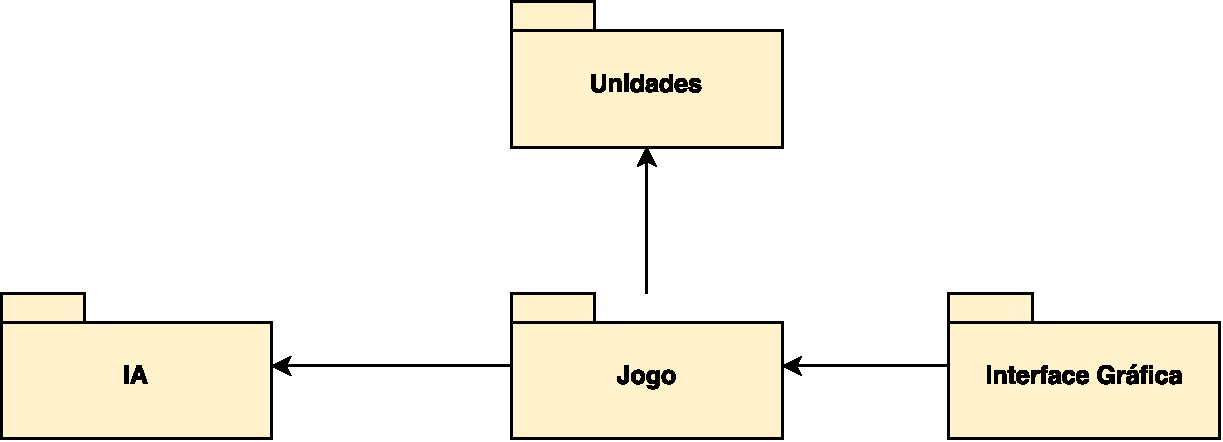
\includegraphics[width=0.4\textwidth]{fig/pacotes.pdf}
	\caption{Arquitetura MicroRTS}
	\label{fig:pacotes}
\end{figure}

O MicroRTS conta com cinco classes principais para funcionamento do jogo e uma para controle da IA. O diagrama de classes presente na Figura~\ref{fig:classes} ilustra os principais métodos das classes originadas do MicroRTS. As funcionalidades de cada classe encontra-se à seguir: 

\begin{itemize}
	\item \textit{GameVisualSimulation} é a interface entre os componentes do jogo e o usuário;
	\item \textit{GameState} e \textit{PhysicalGameState} são responsáveis pelo controle das ações das unidades dentro do mapa;
	\item \textit{UnitTypeTable} é onde cada unidade está associada as ações possíveis no jogo;
	\item \textit{PhysicalGameStatePanel} é responsável pela interface gráfica; e
	\item \textit{IA} é onde a técnica de IA deve ser acoplada ao jogo.
\end{itemize}

\begin{figure}[ht]
	\centering
	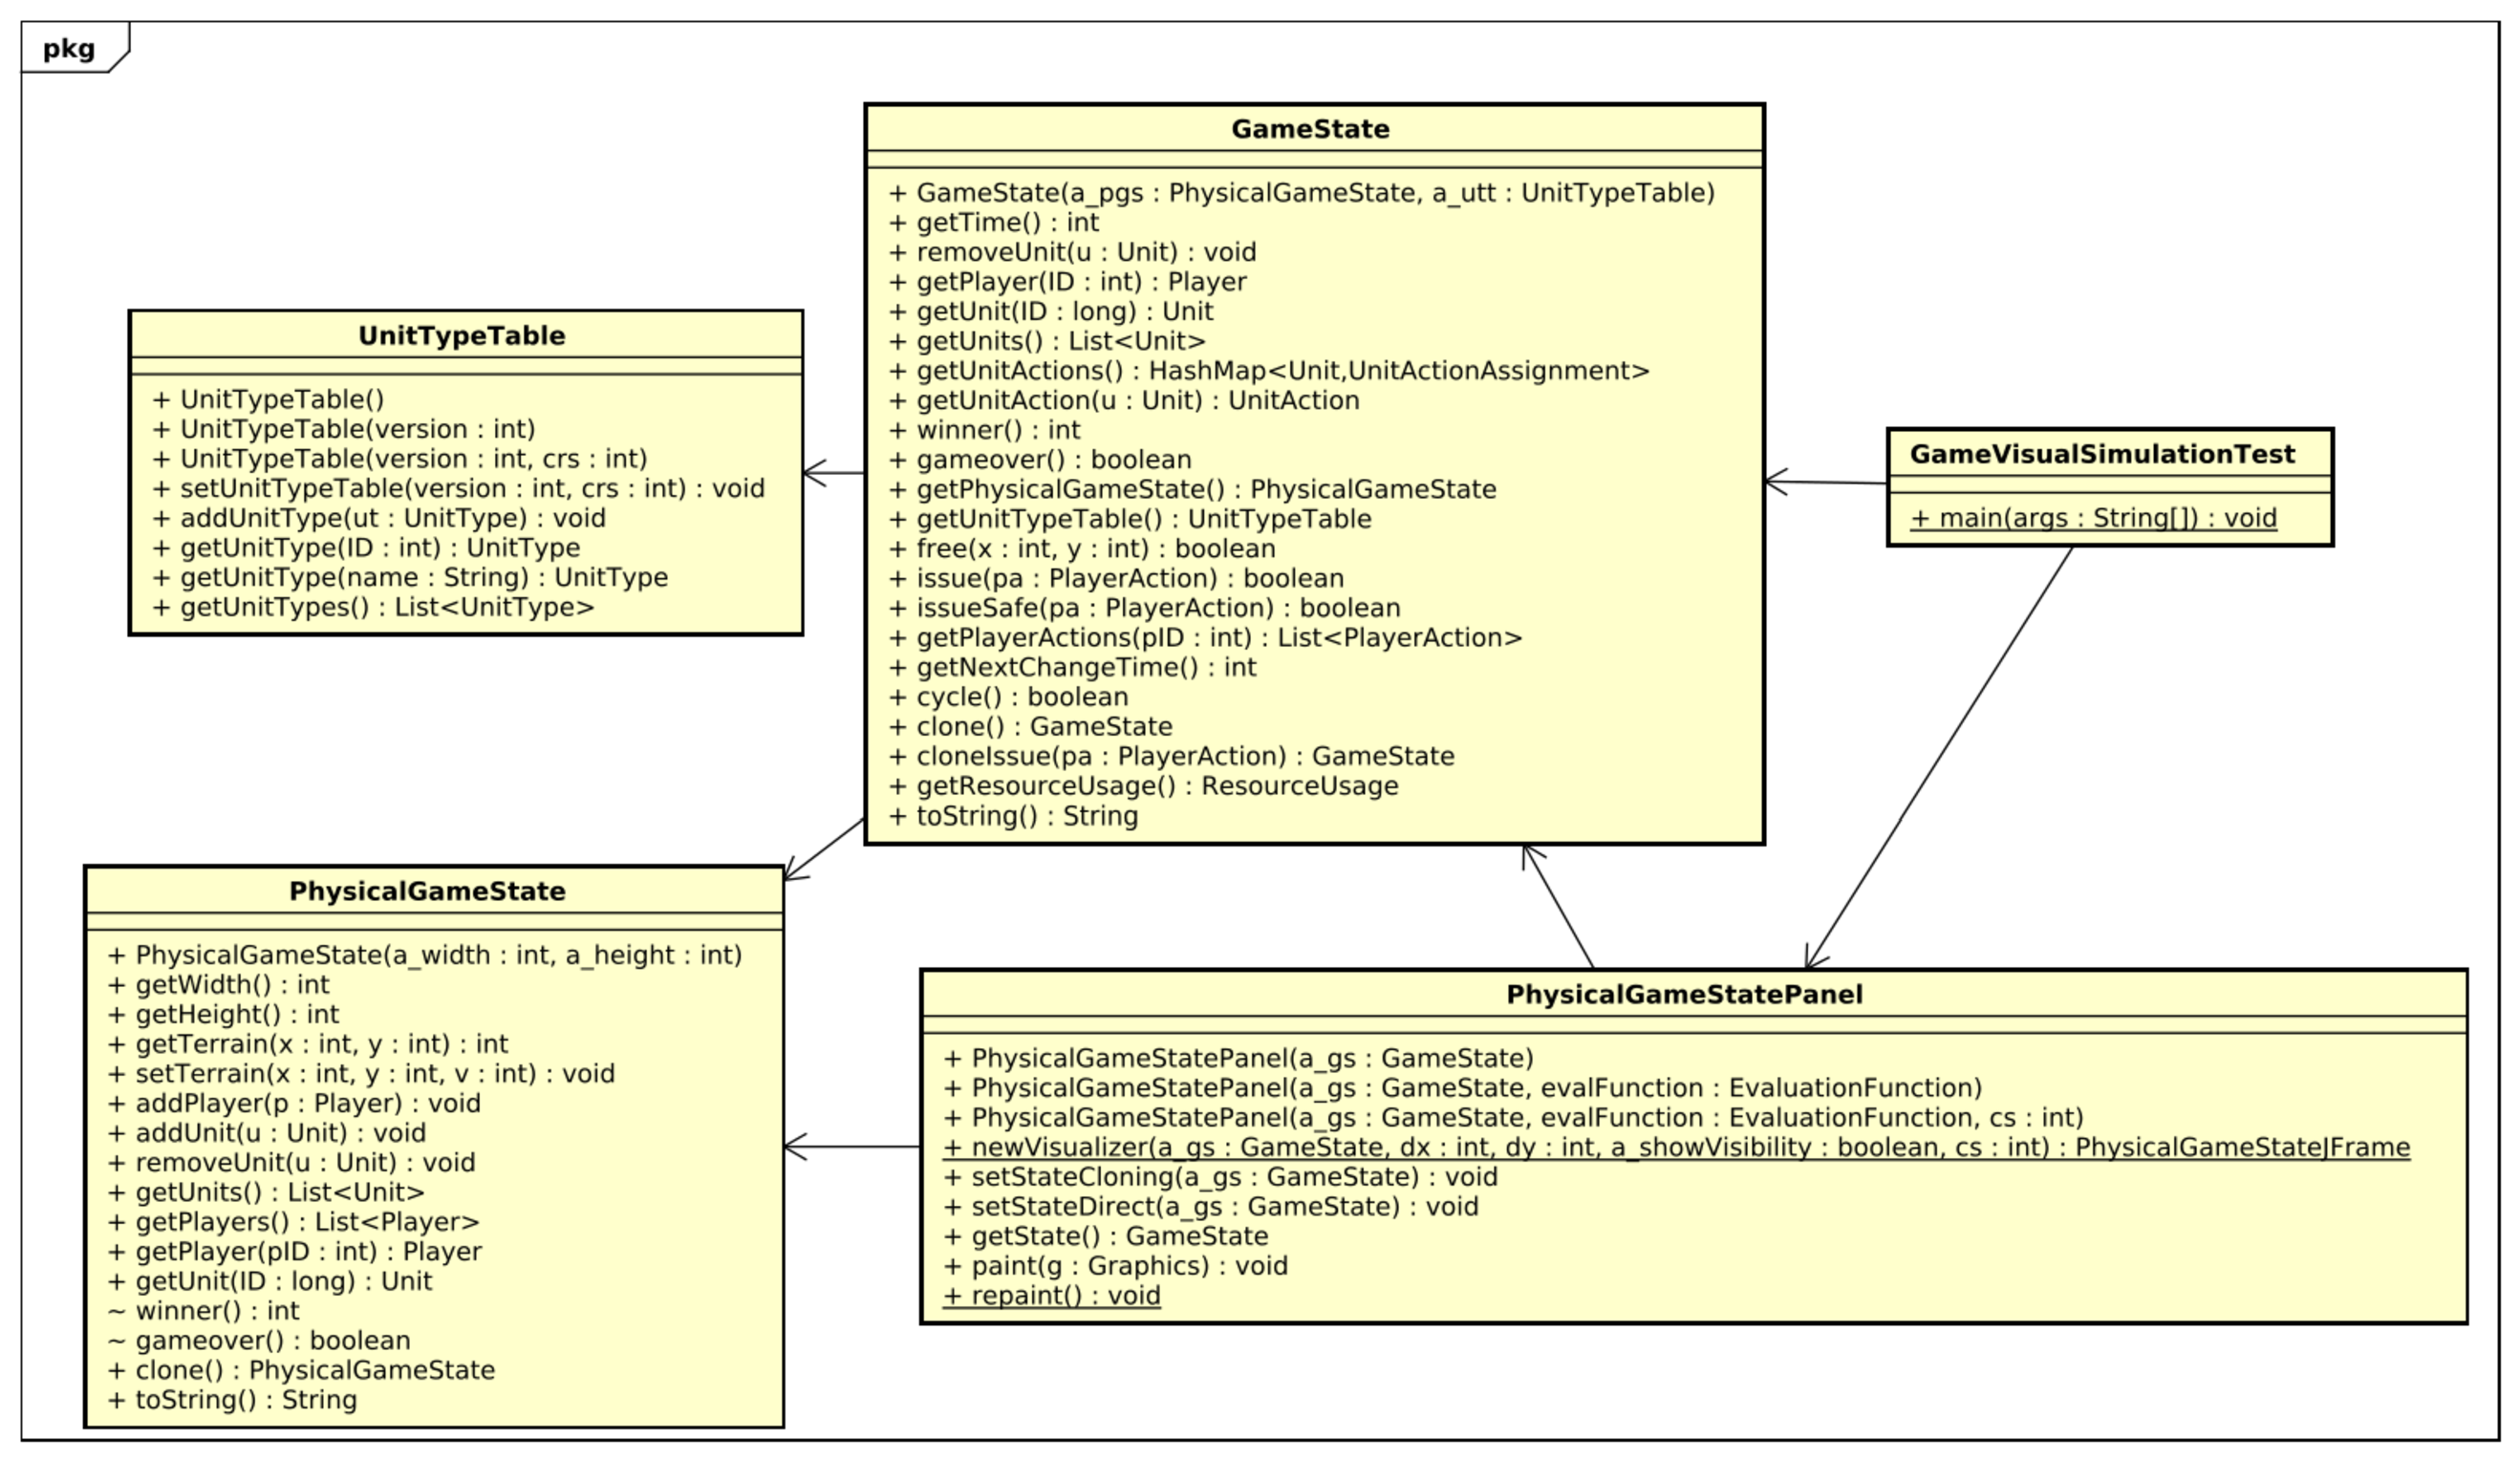
\includegraphics[width=1\textwidth]{fig/classes.pdf}
	\caption{Classes do MicroRTS}
	\label{fig:classes}
\end{figure} 

\subsection{Técnicas de IA}